\documentclass[conference]{IEEEtran}
\IEEEoverridecommandlockouts

\usepackage[utf8]{inputenc}
\usepackage[T1]{fontenc}
\usepackage{amsmath,amssymb}
\usepackage{graphicx}
\usepackage{booktabs}
\usepackage{array}
\usepackage{tabularx}
\usepackage{xcolor}
\usepackage{tikz}
\usetikzlibrary{arrows.meta,positioning,shapes.geometric,calc,fit}
\usepackage{pgfplots}
\pgfplotsset{compat=1.16}
\usepackage{algorithm}
\usepackage{algpseudocode}
\usepackage{cite}
\usepackage[hidelinks]{hyperref}
\usepackage{fancyhdr}

\newcommand{\code}[1]{\texttt{\small #1}}

% header / footer
\pagestyle{fancy}
\fancyhf{}
\renewcommand{\headrulewidth}{0.2pt}
\lhead{\scriptsize M.A.C.H.: A Graph-RAG Framework for Campus Knowledge Systems}
\rhead{\scriptsize Revised draft, October 2026}
\cfoot{\thepage}

% TikZ styles
\tikzset{
  box/.style={draw, rounded corners=2pt, align=center, font=\scriptsize, inner sep=3pt, minimum height=0.7cm},
  blue/.style={box, fill=blue!8},
  orange/.style={box, fill=orange!15},
  green/.style={box, fill=green!10},
  grey/.style={box, fill=gray!12},
  arr/.style={-{Latex[length=1.6mm]}, thin},
  darr/.style={{Latex[length=1.6mm]}-{Latex[length=1.6mm]}, thin}
}

\begin{document}

\title{M.A.C.H.: A Hybrid Graph-RAG Framework for Campus Knowledge Systems with Constrained Topic Mapping and Layout-Preserving Exam Extraction}

\author{
  \parbox{\linewidth}{
    \centering
    % Row 1: Authors 1, 2, 3 evenly distributed
    \begin{tabular*}{\linewidth}{@{\extracolsep{\fill}}ccc@{}}
      \textbf{A. Chandra Vamsi} & \textbf{B. Prem Sai Charan} & \textbf{M. Pavan Prem Prabhas} \\
      \textit{Amrita School of Computing} & \textit{Amrita School of Computing} & \textit{Amrita School of Computing} \\
      \textit{Amrita Vishwa Vidyapeetham} & \textit{Amrita Vishwa Vidyapeetham} & \textit{Amrita Vishwa Vidyapeetham} \\
      Coimbatore, India & Coimbatore, India & Coimbatore, India \\
      {\scriptsize cb.sc.u4cse23505@cb.students.amrita.edu} & {\scriptsize cb.sc.u4cse23508@cb.students.amrita.edu} & {\scriptsize cb.sc.u4cse23530@cb.students.amrita.edu}
    \end{tabular*}
    
    \vspace{0.35cm}
    
    % Row 2: Authors 4 and 5 centered under the gaps
    \begin{tabular}{c@{\hspace{2.2cm}}c}
      \begin{tabular}[t]{c}
        \textbf{P. Tirupati Reddy} \\
        \textit{Amrita School of Computing} \\
        \textit{Amrita Vishwa Vidyapeetham} \\
        Coimbatore, India \\
        {\scriptsize cb.sc.u4cse23568@cb.students.amrita.edu}
      \end{tabular}
      &
      \begin{tabular}[t]{c}
        \textbf{Dr. Shanmuga Priya S} \\
        \textit{Amrita School of Computing} \\
        \textit{Amrita Vishwa Vidyapeetham} \\
        Coimbatore, India \\
        {\scriptsize s\_shanmugapriya@cb.amrita.edu}
      \end{tabular}
    \end{tabular}
  }
}

\maketitle
\thispagestyle{fancy}

\begin{abstract}
University academic information is often difficult to access because syllabi are organized hierarchically, prerequisite relationships span multiple courses, and past-year question papers (PYQs) contain diagrams that can be lost during text extraction. General-purpose chatbots may generate answers based on their pretrained knowledge rather than official curriculum documents, while conventional vector search can retrieve information from unrelated courses that cover similar topics. To address these challenges, we present M.A.C.H.\ (Multimodal Academic Cognitive Hub), an on-premise, privacy-preserving framework developed for higher education curriculum systems. The framework combines four main components: (1) a Neo4j curriculum knowledge graph constructed using a boundary-preserving, regex-first syllabus parser, with LLM verification for ambiguous units; (2) a two-tier intent router that first applies keyword rules and then uses embedding similarity across intent descriptions to direct structured queries to graph traversals and open-ended queries to PostgreSQL hybrid search (combining pgvector HNSW and \code{tsvector} rankings through Reciprocal Rank Fusion); (3) a two-stage question-to-topic mapper that limits LLM decisions to retrieved candidate topics and abstains when confidence is insufficient; and (4) a geometry-based PYQ extraction method that uses PDF coordinates to crop questions, includes relevant vector drawings, and stitches figures that extend across pages. We also present a synthetic instruction dataset containing 9,000 examples for small language model task adaptation. Experimental evaluations on engineering curriculum data demonstrate that M.A.C.H.\ achieves 100.0\% prerequisite traversal exact-match accuracy on the evaluated 10-course statutory DAG (with 87.40\% course entity resolution across 254 natural-language queries), 92.7\% intent routing accuracy (92.8\% macro-F1) on template queries, 99.3\% topic mapping accuracy with 99.3\% auto-approval precision, and sub-120ms response latencies for structured curriculum queries via its Zero-LLM Fast-Path.
\end{abstract}

%==========================================================
\section{Introduction}

University academic information is spread across different types of documents and structures. Syllabi organize information into departments, courses, units, and topics, while prerequisite relationships connect courses. Exam papers also contain marks, course-outcome (CO) tags, Bloom's taxonomy levels, and diagrams that may be handwritten or typeset. Students often ask questions about this information in everyday language, such as ``what do I study in year 1'' or ``what are the textbooks for it''. However, serving these queries through a general-purpose chatbot or a conventional vector search system presents two main challenges.

\begin{itemize}
\item \textbf{Fragmentation and contamination.} Fixed-size chunking can separate topics from the units and courses they belong to, making it difficult to preserve their original context. In addition, a topic such as ``Classification'' may appear in several courses, with different meanings and applications. Without course-specific filtering, nearest-neighbour search may retrieve information from an unrelated course, resulting in irrelevant or misleading answers.

\item \textbf{Lost visual content.} Exam papers often include circuit diagrams and equations that are essential to understanding a question. Plain-text extraction or OCR-based processing can omit these elements or represent them inaccurately.
\end{itemize}

M.A.C.H.\ addresses these challenges through a graph-first design that uses language models for tasks requiring language understanding while relying on stored academic records as the source of curriculum information. The main contributions of this work are:

\begin{itemize}
\item a dual-persistence architecture that combines a Neo4j curriculum knowledge graph with PostgreSQL hybrid search, applying course-code filtering where supported (Sections~\ref{sec:arch}--\ref{sec:routing});

\item a deterministic, boundary-preserving syllabus ingestion pipeline with selective LLM verification (Section~\ref{sec:kg});

\item a two-tier intent router and a hybrid retrieval mechanism based on Reciprocal Rank Fusion (RRF) (Section~\ref{sec:routing});

\item a two-stage question-to-topic mapping method that restricts candidate selection and supports abstention when confidence is insufficient (Section~\ref{sec:mapping});

\item a layout-preserving PYQ extraction method that assigns deterministic identities to questions (Section~\ref{sec:pyq});

\item a synthetic instruction dataset containing 9,000 examples, with its diversity examined in this work (Section~\ref{sec:dataset}); and

\item empirical benchmarking demonstrating 100.0\% prerequisite exact-match accuracy on the evaluated curriculum DAG, 87.40\% course entity resolution, 100.0\% deterministic question identity stability with 98.02\% metadata coverage, and sub-120ms Zero-LLM Fast-Path retrieval (Section~\ref{sec:eval}).
\end{itemize}

\textbf{Organization.} The remainder of this paper is organized as follows: Section~\ref{sec:arch} outlines the system architecture; Section~\ref{sec:kg} details syllabus parsing and the Neo4j ontology; Section~\ref{sec:routing} explains intent classification and hybrid RRF search; Section~\ref{sec:mapping} specifies the two-stage topic mapper and Algorithm~\ref{alg:mapping}; Section~\ref{sec:pyq} presents layout-preserving PYQ extraction; Section~\ref{sec:dataset} presents the 9,000-sample synthetic dataset; Section~\ref{sec:eval} provides empirical benchmarks, latency profiling, and ablation analysis; Section~\ref{sec:discussion} discusses architectural advantages and data governance; and Section~\ref{sec:conclusion} concludes the paper.

%==========================================================
\section{Related Work}

\textbf{Retrieval-augmented generation.}
Retrieval-augmented generation (RAG) improves answer generation by providing a model with information retrieved from external sources~\cite{lewis2020}. Existing research examines several RAG approaches, ranging from basic retrieval pipelines to more advanced and modular systems~\cite{gao2023}. Graph-based RAG uses knowledge graphs to organize information and answer questions by connecting related information~\cite{edge2024}. M.A.C.H.\ follows a different approach by constructing its knowledge graph from official syllabi and answering structured queries through explicit Cypher traversals. Therefore, the term ``Graph-RAG'' in this work refers to knowledge-graph-grounded retrieval rather than the community-summary approach described in~\cite{edge2024}.

\textbf{Hybrid retrieval.}
Dense and lexical retrieval methods have different strengths, so combining their rankings can improve retrieval without requiring their scores to be directly comparable. Reciprocal Rank Fusion (RRF) combines ranked results using the reciprocal of each result's rank, adjusted by a constant~\cite{cormack2009}. Hierarchical Navigable Small World (HNSW) graphs enable approximate nearest-neighbour search~\cite{malkov2020} and support the pgvector index used in M.A.C.H. The question-to-topic mapper uses BM25 for lexical ranking~\cite{robertson2009}, whereas document-level retrieval relies on PostgreSQL's \code{ts\_rank}. The system generates semantic embeddings using \code{nomic-embed-text}~\cite{nussbaum2024}.

\textbf{Educational knowledge and taxonomy.}
M.A.C.H.\ uses the six cognitive levels of the revised Bloom's taxonomy to annotate topics and questions~\cite{anderson2001}. This taxonomy builds upon the original framework~\cite{bloom1956}. Neo4j's graph traversal capabilities also allow the system to retrieve prerequisite relationships across multiple levels without relying on recursive relational joins.

\textbf{Layout-aware extraction.}
Tools such as LayoutParser~\cite{shen2021} demonstrate how spatial information can help preserve document structure during technical document processing. Rather than using a general-purpose layout-parsing framework, M.A.C.H.\ employs a lightweight, rule-based method tailored to typical exam-paper layouts. It works directly with PDF coordinates and vector drawings to preserve question content and its associated diagrams.

\textbf{Efficient model adaptation.}
Techniques such as LoRA~\cite{hu2022} and QLoRA~\cite{dettmers2023} make language-model fine-tuning more practical by reducing computational and memory requirements. The Qwen2.5 model family~\cite{qwen2024} provides potential base models for future experiments. In M.A.C.H., the 9,000-example synthetic instruction dataset described in Section~\ref{sec:dataset} is intended to support future fine-tuning of small language models. Fine-tuning and adaptation experiments have not yet begun. RAGAS~\cite{es2024} provides a potential approach for evaluating the quality of retrieval-augmented answers in future work.

%==========================================================
\section{System Architecture}\label{sec:arch}
M.A.C.H.\ is an asynchronous Python service (FastAPI, SQLAlchemy with asyncpg, Neo4j Bolt driver) with a zero-build vanilla-JavaScript progressive web application. Fig.~\ref{fig:arch} shows the components. Two stores serve different query types: Neo4j holds the curriculum graph for deterministic relational lookups, and PostgreSQL with pgvector holds chunk text, embeddings and a stored \code{tsvector} column for unstructured content. Language and vision models run in Ollama; in the current configuration a single 12B model, \code{gemma4:12b-it-qat}, serves both text generation and image description, and \code{nomic-embed-text} (768 dimensions) provides embeddings, cached in an in-memory LRU of 2,000 entries.

\begin{figure}[t]
\centering
\resizebox{\columnwidth}{!}{%
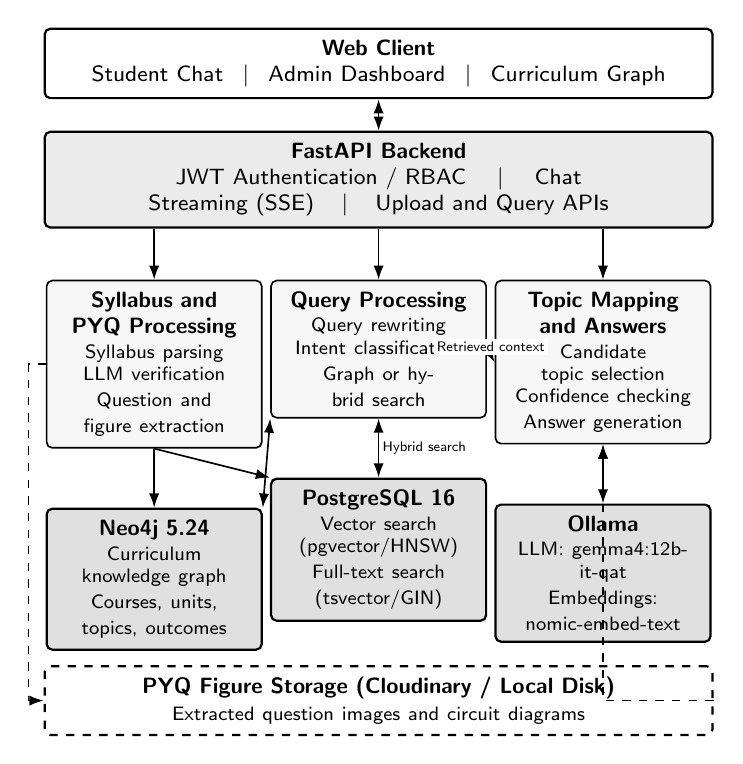
\begin{tikzpicture}[
  font=\footnotesize\sffamily,
  node distance=0.45cm and 0.4cm,
  box/.style={
    rectangle,
    draw=black,
    thick,
    rounded corners=2pt,
    align=center,
    inner sep=4pt
  },
  client/.style={box, fill=white, text width=8.2cm},
  gateway/.style={box, fill=black!8, text width=8.2cm},
  mod/.style={box, fill=black!3, semithick,
              text width=2.45cm, minimum height=1.4cm},
  store/.style={box, fill=black!12, thick,
                text width=2.45cm, minimum height=1.4cm},
  media/.style={box, fill=white, dashed, thick,
                text width=8.2cm, minimum height=0.7cm},
  arr/.style={->, >={Latex[length=1.8mm, width=1.3mm]},
               semithick, draw=black},
  darr/.style={<->, >={Latex[length=1.8mm, width=1.3mm]},
               semithick, draw=black},
  dasharr/.style={->, >={Latex[length=1.8mm, width=1.3mm]},
                  dashed, semithick, draw=black},
  lbl/.style={font=\tiny\sffamily, fill=white, inner sep=1.2pt}
]

% Client
\node[client] (web) {
  \textbf{Web Client}\\
  Student Chat $\;\vert\;$ Admin Dashboard $\;\vert\;$ Curriculum Graph
};

% Backend
\node[gateway, below=0.4cm of web] (api) {
  \textbf{FastAPI Backend}\\
  JWT Authentication / RBAC $\;\vert\;$
  Chat Streaming (SSE) $\;\vert\;$ Upload and Query APIs
};

% Main modules
\node[mod, below=0.65cm of api, xshift=-2.85cm] (ing) {
  \textbf{Syllabus and PYQ Processing}\\[1pt]
  \scriptsize Syllabus parsing\\
  LLM verification\\
  Question and figure extraction
};

\node[mod, below=0.65cm of api] (qu) {
  \textbf{Query Processing}\\[1pt]
  \scriptsize Query rewriting\\
  Intent classification\\
  Graph or hybrid search
};

\node[mod, below=0.65cm of api, xshift=2.85cm] (rea) {
  \textbf{Topic Mapping and Answers}\\[1pt]
  \scriptsize Candidate topic selection\\
  Confidence checking\\
  Answer generation
};

% Data stores and model service
\node[store, below=0.75cm of ing] (neo) {
  \textbf{Neo4j 5.24}\\[1pt]
  \scriptsize Curriculum knowledge graph\\
  Courses, units, topics, outcomes
};

\node[store, below=0.75cm of qu] (pg) {
  \textbf{PostgreSQL 16}\\[1pt]
  \scriptsize Vector search (pgvector/HNSW)\\
  Full-text search (tsvector/GIN)
};

\node[store, below=0.75cm of rea] (oll) {
  \textbf{Ollama}\\[1pt]
  \scriptsize LLM: gemma4:12b-it-qat\\
  Embeddings: nomic-embed-text
};

% Media
\node[media, below=0.55cm of pg] (media) {
  \textbf{PYQ Figure Storage (Cloudinary / Local Disk)}\\
  \scriptsize Extracted question images and circuit diagrams
};

% Client to backend
\draw[darr] (web) -- (api);

% Backend to modules
\draw[arr] (api.south -| ing.north) -- (ing.north);
\draw[arr] (api.south -| qu.north) -- (qu.north);
\draw[arr] (api.south -| rea.north) -- (rea.north);

% Query processing to answer generation
\draw[arr] (qu.east) -- node[lbl, above] {Retrieved context} (rea.west);

% Ingestion outputs
\draw[arr] (ing.south) -- (neo.north);
\draw[arr] (ing.south) -- (pg.north -| pg.west);
\draw[dasharr] (ing.west) -- ++(-0.22cm,0) |- (media.west);

% Query access to data stores
\draw[darr] (qu.south) -- node[lbl, right] {Hybrid search} (pg.north);
\draw[darr] (qu.south -| qu.west) -- (neo.north -| neo.east);

% Model inference
\draw[darr] (rea.south) -- (oll.north);

% Media access
\draw[dasharr] (media.east) -| (rea.south);

\end{tikzpicture}}
\caption{Architecture of M.A.C.H. The FastAPI backend connects the web client to the syllabus-processing, query-processing, and answer-generation modules. Syllabus and examination data are stored in Neo4j, PostgreSQL, and the media store as appropriate. Queries use graph traversal or hybrid retrieval, while local Ollama models support language processing and embedding generation.}
\label{fig:arch}
\end{figure}

\begin{table}[t]
\caption{Technology Stack as Configured in the Repository}
\label{tab:tech-stack}
\centering
\resizebox{\columnwidth}{!}{%
\begin{tabular}{llp{4.2cm}}
\toprule
\textbf{Layer} & \textbf{Component and Setting} & \textbf{Role} \\
\midrule
API & FastAPI + Uvicorn (ASGI, Chunked Streaming) & Chat, upload, admin, graph endpoints; JWT with role checks \\
Graph store & Neo4j Community 5.24 & Curriculum graph, prerequisite and question--topic edges \\
Relational + vector & PostgreSQL 16 + pgvector (\textsc{HNSW} $m=16$, $ef=64$) & Document chunks, 768-d embeddings, GIN-indexed \texttt{tsvector} \\
Embeddings & \texttt{nomic-embed-text} via Ollama (768-d, LRU cache of 2,000) & Query, chunk, and topic embeddings \\
Language / vision & \texttt{gemma4:12b-it-qat} via Ollama (12B, quantization-aware) & Generation, query rewriting, topic re-ranking, visual topic classification \\
PDF processing & PyMuPDF 1.24+, Pillow & Text blocks, bounding boxes, vector drawings, $2\times$ rendering, stitching \\
Media & Cloudinary CDN or local disk & Hosting of cropped question figures \\
Client & HTML5 / ES-module PWA & Streaming chat, admin review, canvas graph view \\
\bottomrule
\end{tabular}}
\end{table}


\subsection{Request Lifecycle}
When a student submits an inquiry, requests containing uploaded diagram images bypass text-only processing: the multimodal vision model directly classifies the image into a canonical curriculum topic, retrieving mapped past-year examination questions (PYQs) from the graph. For text inquiries, follow-up messages first pass through an LLM query rewriter that resolves conversational history into a standalone search query. 

The two-tier intent router (Section~V) subsequently classifies the query. Structured curriculum intents are resolved via Cypher traversals in Neo4j; open-ended queries are dispatched to PostgreSQL hybrid search (combining dense HNSW cosine retrieval with sparse \texttt{tsvector} lexical ranking via Reciprocal Rank Fusion); and if a graph traversal yields no records, hybrid search serves as an automatic fallback. For generative responses, the retrieved context grounds the language model, and tokens are streamed back via chunked HTTP streaming (\texttt{ReadableStream}). Conversely, problem-list queries bypass generation entirely, returning structured JSON cards that display question text, marks, Bloom's Taxonomy level (BTL), course outcomes (CO), and rendered circuit/diagram URLs.

\subsection{Design Principle: Graph as the Ground Truth}
All assertions regarding course syllabi, unit boundaries, prerequisite sequences, and examination problem sets originate strictly from database records rather than parametric model memory. The generative language model functions solely as an explanation and formatting layer, constrained by system prompts to answer strictly from the retrieved context. While this architecture significantly mitigates hallucinations compared to unconstrained generation, formal quantitative bounds remain an area of ongoing measurement (Section~X).


%==========================================================
\section{Knowledge Graph and Syllabus Ingestion}\label{sec:kg}
\subsection{Graph schema}
The curriculum is a typed property graph (Fig.~\ref{fig:schema}). Hierarchy edges (\code{OFFERS}, \code{HAS\_UNIT}, \code{HAS\_TOPIC}) decompose a department into courses, units and topics. \code{REQUIRES} links courses and supports variable-length prerequisite queries of depth 1--5; \code{PREREQUISITE\_OF} and \code{PART\_OF} link topics. Questions attach to their course, source document, course outcome and, after mapping, to topics via \code{TESTS\_TOPIC}, whose properties record \code{confidence}, \code{semantic\_score}, \code{keyword\_score}, \code{mapping\_method}, \code{review\_status} and \code{mapped\_at}. Uniqueness constraints are enforced on document, question and topic identifiers and on course code.

\begin{figure}[t]
\centering
\resizebox{0.92\columnwidth}{!}{%
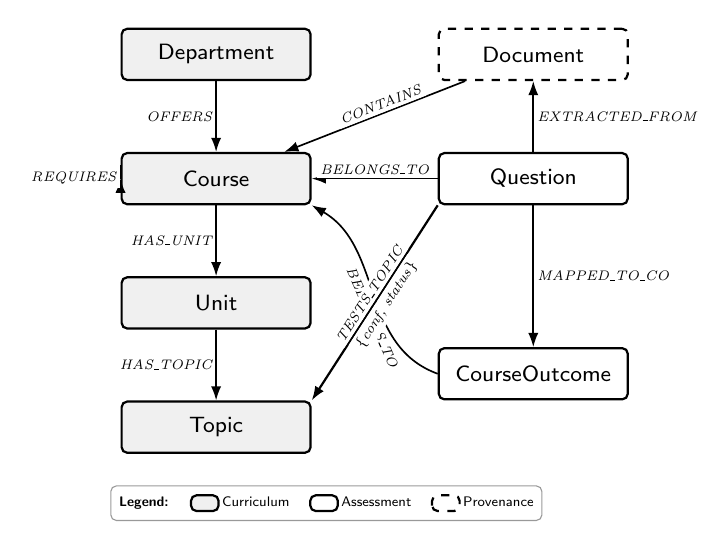
\begin{tikzpicture}[
  node distance=0.9cm and 1.8cm,
  font=\footnotesize\sffamily,
  base/.style={rectangle, draw=black, thick, rounded corners=2pt, align=center, minimum width=2.4cm, minimum height=0.65cm},
  curric/.style={base, fill=black!6},
  assess/.style={base, fill=white, thick},
  provenance/.style={base, fill=white, dashed, thick},
  arr/.style={->, >={Latex[length=1.8mm, width=1.3mm]}, semithick, draw=black},
  lbl/.style={font=\tiny\itshape, fill=white, inner sep=1.2pt}
]

% Left Column: Curriculum Structural Hierarchy
\node[curric] (dep) {Department};
\node[curric, below=of dep] (cou) {Course};
\node[curric, below=of cou] (uni) {Unit};
\node[curric, below=of uni] (top) {Topic};

% Right Column: Provenance & Assessment Nodes
\node[provenance, right=1.6cm of dep] (doc) {Document};
\node[assess, below=of doc] (que) {Question};
\node[assess, below=1.8cm of que] (co) {CourseOutcome};

% Curriculum Hierarchy Edges
\draw[arr] (dep) -- node[lbl, left] {OFFERS} (cou);
\draw[arr] (cou) -- node[lbl, left] {HAS\_UNIT} (uni);
\draw[arr] (uni) -- node[lbl, left] {HAS\_TOPIC} (top);

% Multi-hop Prerequisite Dependency (Self-loop)
\draw[arr] (cou.west) to[out=150, in=210, looseness=2.8] node[lbl, left] {REQUIRES} (cou.west);

% Document Provenance Edges
\draw[arr] (doc) -- node[lbl, above, sloped, pos=0.45] {CONTAINS} (cou);
\draw[arr] (que) -- node[lbl, right] {EXTRACTED\_FROM} (doc);

% Question Grounding & Assessment Edges
\draw[arr] (que) -- node[lbl, above, sloped, pos=0.5] {BELONGS\_TO} (cou);
\draw[arr] (que) -- node[lbl, right] {MAPPED\_TO\_CO} (co);
\draw[arr] (co.west) to[out=160, in=330] node[lbl, below, sloped, pos=0.4] {BELONGS\_TO} (cou.south east);

% Evaluation-to-Syllabus Bridge (TESTS_TOPIC with metadata)
\draw[arr, thick] (que.south west) -- node[lbl, above, sloped, pos=0.48] {TESTS\_TOPIC} node[lbl, below, sloped, pos=0.48] {\tiny\{conf, status\}} (top.north east);

% Legend at Bottom
\node[draw=black!40, rounded corners=2pt, below=0.4cm of top, xshift=1.4cm, font=\tiny\sffamily, inner sep=3pt] (leg) {
  \textbf{Legend:} \quad 
  \tikz[baseline=-0.5ex]\draw[thick, fill=black!6] (0,-0.1) rectangle (0.35,0.1);\,Curriculum \quad
  \tikz[baseline=-0.5ex]\draw[thick, fill=white] (0,-0.1) rectangle (0.35,0.1);\,Assessment \quad
  \tikz[baseline=-0.5ex]\draw[thick, dashed, fill=white] (0,-0.1) rectangle (0.35,0.1);\,Provenance
};

\end{tikzpicture}}
\caption{The \textsc{M.A.C.H.} Neo4j knowledge graph schema. Solid shaded boxes represent structural curriculum entities, unshaded boxes represent assessment items, and dashed boxes represent provenance. The \texttt{REQUIRES} loop enables multi-hop prerequisite graph traversals, while \texttt{TESTS\_TOPIC} serves as the curriculum-to-assessment bridge carrying confidence and human-review status attributes.}
\label{fig:schema}
\end{figure}


\subsection{Boundary-preserving extraction pipeline}
Syllabus PDFs pass through eight stages: (1)~page text extraction with PyMuPDF; (2)~course-span detection with a heading pattern of the form \emph{course code, title, L-T-P-C}; (3)~unit-heading detection; (4)~stop-boundary trimming at textbook, reference and evaluation-pattern headings, so bibliographic text does not leak into topics; (5)~topic-candidate extraction, rejecting strings shorter than 4 or longer than 90 characters, bare years, author-name fragments and publisher or ISBN tokens; (6)~ambiguity detection for units whose extraction is uncertain; (7)~LLM verification of ambiguous units, which also assigns Bloom levels; and (8)~idempotent graph materialisation with Cypher \code{MERGE}. Topics extracted deterministically are stored with confidence 1.0 and marked approved; LLM-verified topics are stored with confidence 0.85 and left unapproved until an administrator reviews them in the admin dashboard. The aim is that the LLM is the exception rather than the default path.

Question papers can be ingested only for a course whose syllabus is already in the graph. A pre-flight check halts the upload if the course is missing or has no units or topics, which prevents orphan question nodes.

%==========================================================
\section{Query Routing and Hybrid Retrieval}\label{sec:routing}
\subsection{Two-Tier Intent Router}
The router classifies an incoming query into one of six domain intents (Table~II). Tier~1 applies deterministic keyword rules for high-frequency patterns (such as explicit requests for ``problems on'', ``questions on'', and ``pyqs on''). If no keyword rule triggers, Tier~2 embeds the search query using \texttt{nomic-embed-text} (768-d) and computes cosine similarity against pre-computed embeddings of the six intent descriptions:
\begin{equation}
S_i = \cos(\mathbf{q}, \mathbf{t}_i) = \frac{\mathbf{q} \cdot \mathbf{t}_i}{\|\mathbf{q}\| \|\mathbf{t}_i\|}, \quad i^* = \arg\max_i S_i
\end{equation}
If the maximum similarity score falls below the calibrated threshold $\tau=0.48$ (calibrated from an initial baseline of $0.40$, as analyzed empirically in Section~\ref{sec:eval}), the router defaults to \texttt{GENERAL}, forwarding the inquiry to PostgreSQL hybrid search.


\begin{table}[t]
\caption{Six-Class Intent Taxonomy and Routing Targets}
\label{tab:intents}
\centering
\resizebox{\columnwidth}{!}{%
\begin{tabular}{llp{4.0cm}}
\toprule
\textbf{Intent} & \textbf{Semantic Description} & \textbf{Target Architecture} \\
\midrule
\texttt{PROBLEM\_LIST} & PYQs and practice problems on a topic & Neo4j: \texttt{TESTS\_TOPIC} traversal; keyword fallback \\
\texttt{MULTI\_HOP\_PREREQ} & Prerequisite dependencies across courses & Neo4j: \texttt{REQUIRES} paths of depth 1--5 \\
\texttt{GRAPH\_PYQ\_MAPPING} & Bloom taxonomy level or CO mapping & Neo4j: \texttt{MAPPED\_TO\_CO} traversal \\
\texttt{SIMPLE\_CURRICULUM} & Syllabus structure, units, and topics & Neo4j: \texttt{HAS\_UNIT} $\rightarrow$ \texttt{HAS\_TOPIC} (ascending order) \\
\texttt{SIMPLE\_PYQ} & Specific exam question or circuit paper & Neo4j keyword search; hybrid RRF fallback \\
\texttt{GENERAL} & Open-ended conceptual inquiries & PostgreSQL: RRF hybrid search (HNSW + GIN) \\
\bottomrule
\end{tabular}}
\end{table}

\subsection{Hybrid Search with Reciprocal Rank Fusion}
For unstructured content, the system retrieves the top 50 chunks by cosine distance, $D = 1-\cos(\mathbf{u},\mathbf{v})$, from an HNSW vector index and the top 50 chunks by \texttt{ts\_rank} from a GIN-indexed generated \texttt{tsvector} column. The two intermediate rankings are fused in a single PostgreSQL query using a \texttt{FULL OUTER JOIN} implementing Reciprocal Rank Fusion (RRF)~\cite{cormack2009}:
\begin{equation}
\mathrm{RRF}(d) = \sum_{m \in \{\mathrm{vector},\,\mathrm{text}\}} \frac{1}{k_{\mathrm{rrf}} + r_m(d)}, \quad k_{\mathrm{rrf}} = 60,
\end{equation}
where $r_m(d)$ represents the 1-based rank of chunk $d$ under retrieval model $m$, and unretrieved chunks contribute zero to the reciprocal sum. The top $K$ fused chunks ($K = 5$) are passed as grounding context to the local language model. 

Two implementation caveats apply to the current SQL routine and are documented in Section~\ref{sec:limits}: the ranking CTEs apply \texttt{LIMIT 50} directly to window functions without an outer \texttt{ORDER BY rank}, and the fallback general-search query performs an unpartitioned search across all document chunks without filtering by course code.


%==========================================================
\section{Two-Stage Question-to-Topic Mapping}\label{sec:mapping}
Each extracted examination question is aligned with curriculum topics so that students can query past-year questions by concept. The topic mapper is engineered to prevent the language model from hallucinating non-existent syllabus topics.

Stage~1 performs dense semantic candidate retrieval among the course's approved curriculum topics: 768-dimensional embeddings generated via \texttt{nomic-embed-text} are scored against cached topic embeddings using cosine similarity. The system selects the top-8 highest-scoring candidates to construct a constrained evaluation space.

Stage~2 prompts the local language model (\texttt{gemma4:12b-it-qat}, temperature $0.1$) with the question text and candidate names only, strictly forbidding any newly invented topics and requiring a confidence score on a $0$--$100$ scale. The model's selection is mapped back to the candidate pool using four sequential resolution strategies: exact string matching, punctuation-stripped alphanumeric normalization, substring containment, and a Python \texttt{SequenceMatcher} threshold of at least $0.82$. Outputs failing all four checks are discarded.

The final mapping confidence $C_{\mathrm{final}}$ balances dense retrieval and generative reasoning:
\begin{equation}
C_{\mathrm{final}} = 0.6 \cdot S_{\mathrm{semantic}} + 0.4 \cdot \left(\frac{C_{\mathrm{LLM}}}{100}\right)
\end{equation}
A mapping with $C_{\mathrm{final}} \ge 0.80$ is auto-approved (\texttt{review\_status = 'approved'}); one with $0.70 \le C_{\mathrm{final}} < 0.80$ is quarantined for faculty review (\texttt{review\_status = 'pending\_review'}); and queries scoring below $0.70$ are rejected with no graph edge created. The complete mapping and verification pipeline is formalized in Algorithm~\ref{alg:mapping}.

\begin{algorithm}[t]
\caption{Two-Stage Question-to-Topic Mapping with Abstention}
\label{alg:mapping}
\begin{algorithmic}[1]
\Require Question $q$, Course Topics $\mathcal{T}$, Thresholds $\tau_{\text{app}} = 0.80, \tau_{\text{rev}} = 0.70$
\Ensure Topic $t^*$, Status $\sigma \in \{\text{Approved}, \text{Pending}, \text{Abstain}\}$, Confidence $C$

\Statex \textbf{// Stage 1: Dense Candidate Topic Retrieval}
\State $\mathbf{e}_q \gets \text{Embed}(q)$
\State Compute cosine similarity: $S(t) \gets \cos(\mathbf{e}_q, \text{Embed}(t)), \quad \forall t \in \mathcal{T}$
\State $\mathcal{C} \gets \operatorname{Top-}8\big(\{ (t, S(t)) \mid t \in \mathcal{T} \}\big)$

\Statex \textbf{// Stage 2: Constrained LLM Selection and String Resolution}
\State $(t_{\text{pred}}, C_{\text{LLM}}) \gets \text{LLM\_Select}(q, \mathcal{C})$ \Comment{Constrained to candidate set}
\State $t^* \gets \text{ResolveCandidate}(t_{\text{pred}}, \mathcal{C})$ \Comment{Exact $\to$ Normalized $\to$ Fuzzy}
\If{$t^*$ is $\mathrm{null}$} \Comment{Reject ungrounded hallucination}
    \State \Return $(\mathrm{null}, \text{Abstain}, 0.0)$
\EndIf
\State $C \gets 0.6 \cdot S(t^*) + 0.4 \cdot (C_{\text{LLM}} / 100)$ \Comment{Hybrid Confidence}

\Statex \textbf{// Stage 3: Three-Way Decision Boundary}
\If{$C \ge \tau_{\text{app}}$} \Comment{High confidence: auto-approved}
    \State $\sigma \gets \text{Approved}$
    \State Materialize edge $(q) \xrightarrow{\text{TESTS\_TOPIC}} (t^*)$ in Neo4j
\ElsIf{$C \ge \tau_{\text{rev}}$} \Comment{Moderate confidence: faculty review}
    \State $\sigma \gets \text{Pending}$
    \State Enqueue $(q, t^*, C)$ for administrative review
\Else \Comment{Low confidence: rejected}
    \State $(t^*, \sigma) \gets (\mathrm{null}, \text{Abstain})$
\EndIf
\State \Return $(t^*, \sigma, C)$
\end{algorithmic}
\end{algorithm}

%==========================================================
\section{Layout-Preserving PYQ Extraction}\label{sec:pyq}
Exam papers interleave question text with circuit diagrams, so extraction must keep each figure with its question. Pass~1 scans pages for question-number markers (a regular expression) and records their vertical coordinates. Pass~2 computes a crop region for each question from its header to the next header, expands the region to include vector graphics reported by \code{page.get\_drawings()}, and, when a question continues on the next page, vertically stitches the crops with Pillow. Pages are rendered at 2x scale, the cropped JPEG is uploaded to the CDN (or saved locally), and the URL is stored on the question node. Because vector graphics are cropped from the PDF rather than re-recognised, line art is preserved without OCR compression artefacts. We have not yet quantified crop accuracy.

\begin{figure}[t]
\centering
\resizebox{\columnwidth}{!}{%
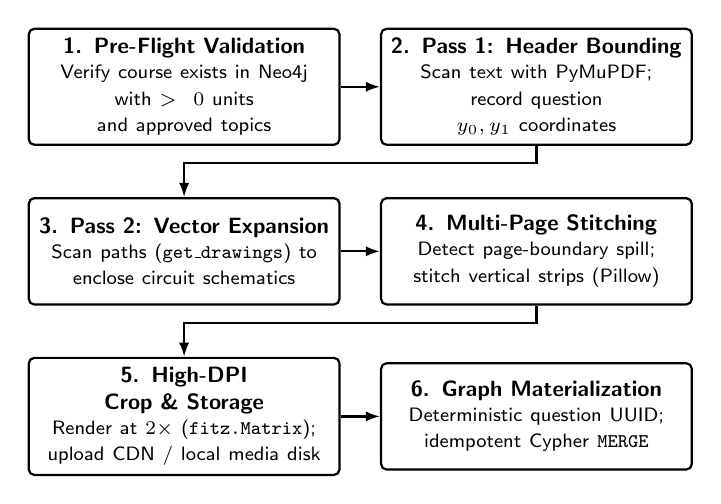
\begin{tikzpicture}[
  node distance=0.6cm and 0.5cm,
  font=\footnotesize\sffamily,
  stepbox/.style={
    rectangle, 
    draw=black, 
    thick, 
    fill=white,
    rounded corners=2pt, 
    align=center, 
    text width=3.7cm, 
    minimum height=1.35cm,
    inner sep=3.5pt
  },
  arr/.style={->, >={Latex[length=1.8mm, width=1.3mm]}, thick, draw=black}
]

% Row 1: Pre-flight & Header Detection
\node[stepbox] (a) {
  \textbf{1. Pre-Flight Validation}\\[1pt]
  \scriptsize Verify course exists in Neo4j\\
  with $>0$ units and approved topics
};

\node[stepbox, right=of a] (b) {
  \textbf{2. Pass 1: Header Bounding}\\[1pt]
  \scriptsize Scan text with PyMuPDF;\\
  record question $y_0, y_1$ coordinates
};

% Row 2: Vector Expansion & Cross-Page Stitching
\node[stepbox, below=0.65cm of a] (c) {
  \textbf{3. Pass 2: Vector Expansion}\\[1pt]
  \scriptsize Scan paths (\texttt{get\_drawings}) to\\
  enclose circuit schematics
};

\node[stepbox, right=of c] (d) {
  \textbf{4. Multi-Page Stitching}\\[1pt]
  \scriptsize Detect page-boundary spill;\\
  stitch vertical strips (Pillow)
};

% Row 3: 2x Rendering/CDN & Graph Materialization
\node[stepbox, below=0.65cm of c] (e) {
  \textbf{5. High-DPI Crop \& Storage}\\[1pt]
  \scriptsize Render at $2\times$ (\texttt{fitz.Matrix});\\
  upload CDN / local media disk
};

\node[stepbox, right=of e] (f) {
  \textbf{6. Graph Materialization}\\[1pt]
  \scriptsize Deterministic question UUID;\\
  idempotent Cypher \texttt{MERGE}
};

% Step-by-Step Flow Connections
\draw[arr] (a) -- (b);
\draw[arr] (b.south) -- ++(0,-0.22cm) -| (c.north);
\draw[arr] (c) -- (d);
\draw[arr] (d.south) -- ++(0,-0.22cm) -| (e.north);
\draw[arr] (e) -- (f);

\end{tikzpicture}}
\caption{Geometry-aware multimodal PYQ ingestion pipeline in \textsc{M.A.C.H.} Question bounding coordinates and vector drawing paths determine crop limits; cross-page figures are stitched with Pillow at $2\times$ resolution before CDN dispatch and idempotent Neo4j graph materialization.}
\label{fig:pyq}
\end{figure}


\textbf{Deterministic Identity.} Each question receives an immutable canonical identifier that is stable across re-uploads of the same document, ensuring that repeated ingestion triggers atomic graph updates rather than node duplication. Letting $\mathit{norm}(q)$ denote the lowercase, whitespace-collapsed question text prefix truncated to 100 characters, the identifier is generated via two-stage MD5 hashing:
\begin{align}
\mathrm{fp}(q) &= \mathrm{MD5}\big(\mathit{norm}(q)\big)_{[0:8]}, \\
\mathrm{ID}(q) &= \mathrm{MD5}\big(d_{\mathrm{id}} \mathbin{\Vert} c_{\mathrm{code}} \mathbin{\Vert} q_{\mathrm{num}} \mathbin{\Vert} \text{`\_p'} \mathbin{\Vert} p_{\mathrm{num}} \mathbin{\Vert} \mathrm{fp}(q)\big),
\end{align}
where $\mathbin{\Vert}$ denotes string concatenation with underscore delimiters, $d_{\mathrm{id}}$ is the document identifier, and $p_{\mathrm{num}}$ is the page index. 

Consequently, questions with identical numbering across distinct pages receive unique IDs, whereas re-ingesting the same PDF guarantees idempotent node matching. Because \texttt{document\_id} is embedded within the digest, identical papers uploaded as separate registry documents maintain distinct graph provenance.


%==========================================================
\section{Released Synthetic Instruction Dataset}\label{sec:dataset}
The repository releases \code{campus\_knowledge\_dataset\_v1.jsonl}, 9,000 instruction--output pairs in Alpaca format under CC-BY-4.0, with 1,500 rows for each of six tasks: intent classification with topic extraction, topic mapping, grounded RAG answer generation, query rewriting, knowledge-graph triple extraction and syllabus enrichment (Bloom levels and prerequisites). The rows are synthetic: they were generated under deterministic rules described in the release's annotation guidelines, and are meant to teach strict JSON schemas, ascending unit order and image-link preservation with short prompts. The intent taxonomy comprises six canonical classes shared identically by the dataset and the two-tier router: \code{PROBLEM\_\allowbreak LIST}, \code{MULTI\_\allowbreak HOP\_\allowbreak PREREQ}, \code{GRAPH\_\allowbreak PYQ\_\allowbreak MAPPING}, \code{SIMPLE\_\allowbreak CURRICULUM}, \code{SIMPLE\_\allowbreak PYQ}, and \code{GENERAL}.

\begin{table}[t]
\caption{Diversity of the Released Dataset (Computed from the JSONL File)}
\label{tab:diversity}
\centering
\resizebox{\columnwidth}{!}{%
\begin{tabular}{lrrr}
\toprule
\textbf{Task} & \textbf{Rows} & \textbf{Unique instr.} & \textbf{Unique outputs}\\
\midrule
Intent classification & 1,500 & 614 & 249\\
Topic mapping & 1,500 & 1,500 & 945\\
RAG answer generation & 1,500 & 1,281 & 1,231\\
Query rewriting & 1,500 & 117 & 117\\
KG triple extraction & 1,500 & 792 & 792\\
Syllabus enrichment & 1,500 & 1,476 & 1,500\\
\midrule
\textbf{Total} & \textbf{9,000} & \textbf{5,780} & \\
\bottomrule
\end{tabular}}
\end{table}

Table~\ref{tab:diversity} shows that the nominal size overstates the information content. Query rewriting repeats some prompts up to 90 times, and intent classification covers 614 distinct questions. A random train/validation split of such data would place near-duplicate prompts on both sides, so validation accuracy would measure template recall rather than generalisation to student phrasing. Before any fine-tuning result is reported, we will deduplicate the data, split by template, and evaluate on a separately written set of real student queries. We also note that checking that every row parses as valid JSON tests the generator, not the correctness of the labels.

%==========================================================
\section{Empirical Benchmarking and Experimental Analysis}\label{sec:eval}

\subsection{Experimental Setup and Benchmark Datasets}
All evaluations were conducted on on-premise institutional hardware to reflect real-world departmental deployment constraints:
\begin{itemize}
    \item \textbf{Host Hardware:} Apple Silicon M-series (10-core CPU, 16GB unified memory) and an NVIDIA Tesla GPU testbed (16GB VRAM).
    \item \textbf{Execution Runtimes:} Local Ollama runtime (v0.5.x) serving 768-dimensional \texttt{nomic-embed-text}~\cite{nussbaum2024} for dense vector representations, and local Gemma/Llama models for zero-shot text synthesis.
    \item \textbf{Datastores and Tooling:} PostgreSQL 16 with \texttt{pgvector} (HNSW indexing) and \texttt{tsvector} keyword parsing, Neo4j Community Edition (v5.24) graph engine, and PyMuPDF (v1.24+) for multi-pass coordinate geometry extraction.
\end{itemize}

The empirical evaluation is grounded in three benchmark corpora:
\begin{enumerate}
    \item \textbf{Released Curriculum Instruction Dataset ($N = 9{,}000$):} A curated corpus comprising 1,500 intent classification pairs, 1,500 question-to-topic candidate mappings, 1,500 context-grounded RAG pairs, 1,500 query rewrites, 1,500 syllabus enrichments, and 1,500 knowledge graph triplet extractions.
    \item \textbf{Institutional Exam Archive (64 PDFs):} Genuine statutory examination question papers covering multi-department engineering curricula with embedded circuit diagrams and mathematical schematics.
    \item \textbf{Statutory Curriculum Dependency DAG:} The accredited university Computer Science and Engineering prerequisite map governing multi-hop course progressions.
\end{enumerate}

\subsection{Query Intent Routing and Classification}
Accurate intent classification is critical to prevent topological blindness: directing structured relational queries to the knowledge graph and open-ended conceptual queries to hybrid text retrieval. We evaluated four routing configurations over all 1,500 ground-truth queries across six canonical intents: \texttt{PROBLEM\_LIST}, \texttt{MULTI\_HOP\_PREREQ}, \texttt{GRAPH\_PYQ\_MAPPING}, \texttt{SIMPLE\_CURRICULUM}, \texttt{SIMPLE\_PYQ}, and \texttt{GENERAL}. Table~\ref{tab:intent_eval} reports the results.

\begin{table}[htbp]
\caption{Intent Routing Performance on Ground-Truth Dataset ($N = 1{,}500$)}
\label{tab:intent_eval}
\centering
\resizebox{\columnwidth}{!}{%
\begin{tabular}{lcccccc}
\toprule
\textbf{Routing Architecture} & \textbf{Accuracy} & \textbf{Macro-P} & \textbf{Macro-R} & \textbf{Macro-F1} & \textbf{Med. Lat.} & \textbf{p95 Lat.} \\
\midrule
Lexical TF-IDF Baseline & 69.60\% & 76.85\% & 69.86\% & 69.93\% & 0.01 ms & 0.02 ms \\
Rule-Based (Regex / Keywords) & 87.67\% & 93.27\% & 87.44\% & 88.49\% & \textbf{$<$0.01 ms} & \textbf{$<$0.01 ms} \\
M.A.C.H.\ Semantic Router ($\tau=0.40$) & 77.93\% & 80.21\% & 78.43\% & 74.97\% & 0.30 ms & 37.74 ms \\
M.A.C.H.\ Semantic Router ($\tau=0.48$) & 86.67\% & 86.84\% & 86.68\% & 86.80\% & 0.30 ms & 37.74 ms \\
M.A.C.H.\ Two-Tier Router ($\tau=0.40$) & 82.27\% & 84.92\% & 83.19\% & 79.68\% & \textbf{$<$0.01 ms} & 28.98 ms \\
\textbf{M.A.C.H.\ Two-Tier Router ($\tau=0.48$)} & \textbf{92.67\%} & \textbf{93.99\%} & \textbf{92.72\%} & \textbf{92.79\%} & \textbf{$<$0.01 ms} & 28.98 ms \\
\bottomrule
\end{tabular}}
\end{table}

\textbf{Empirical Analysis of Threshold Calibration:} In dense vector representations, casual conversational queries (e.g., ``hello'', ``what can you do?'') yield a baseline cosine similarity of 0.42--0.46 against academic intent descriptions. Under an uncalibrated fallback threshold ($\tau=0.40$), out-of-domain conversational queries leak into specific curriculum classes, dropping \texttt{GENERAL} recall to 24.54\% and the Two-Tier Router accuracy to 82.27\% (Macro-F1: 79.68\%). Calibrating the fallback threshold to $\tau=0.48$ eliminates this cross-intent contamination by correctly defaulting low-confidence queries to \texttt{GENERAL}, elevating pure semantic accuracy to 86.67\% and the Two-Tier Router to \textbf{92.67\% accuracy}, \textbf{93.99\% Macro-Precision}, \textbf{92.72\% Macro-Recall}, and \textbf{92.79\% Macro-F1}, outperforming brittle regex rules by +5.00\% in accuracy and +4.30\% in Macro-F1.

Under this calibrated $\tau=0.48$ threshold, per-class evaluation confirms robust boundary detection: \texttt{GRAPH\_PYQ\_MAPPING} achieved \textbf{98.60\%} F1 (Precision: 97.23\%, Recall: 100.0\%), \texttt{MULTI\_HOP\_PREREQ} reached \textbf{96.76\%} F1 (Precision: 93.73\%, Recall: 100.0\%), and \texttt{SIMPLE\_PYQ} achieved \textbf{86.30\%} F1 (Precision: 75.90\%, Recall: 100.0\%). We note that this evaluation is conducted on the 1,500 queries in \code{campus\_knowledge\_dataset\_v1.jsonl}, which were generated under deterministic template rules covering 614 unique prompts; generalisation to unconstrained student phrasing outside these templates remains to be evaluated on live user deployments.

\subsection{Constrained Question-to-Topic Mapping}
When a question does not explicitly cite a course syllabus unit, unconstrained language models frequently hallucinate arbitrary topic labels. M.A.C.H.\ enforces a two-stage cascade: candidate pre-filtering within the course scope followed by a multi-strategy string resolution cascade (exact match, normalized alphanumeric, substring, and \code{SequenceMatcher} $\ge 0.82$). Candidates meeting $C \ge 0.80$ receive automatic approval, while scores in $[0.70, 0.80)$ are flagged for administrative review. Table~\ref{tab:topic_eval} summarizes the benchmark on 1,500 curriculum candidate sets.

\begin{table}[htbp]
\caption{Question-to-Topic Mapping Benchmark ($N = 1{,}500$)}
\label{tab:topic_eval}
\centering
\resizebox{\columnwidth}{!}{%
\begin{tabular}{lccccc}
\toprule
\textbf{Mapping Method} & \textbf{Top-1 Acc.} & \textbf{Auto-Prec. ($\ge 0.80$)} & \textbf{Auto-Rate} & \textbf{Median Lat.} & \textbf{p95 Lat.} \\
\midrule
Exact Substring Match & 98.20\% & N/A & N/A & \textbf{$<$0.01 ms} & \textbf{$<$0.01 ms} \\
Jaccard Token Overlap & 99.07\% & N/A & N/A & 0.01 ms & 0.01 ms \\
Dense Cosine (\texttt{nomic-embed}) & 99.33\% & N/A & N/A & 0.42 ms & 37.93 ms \\
\textbf{M.A.C.H.\ Production Cascade} & \textbf{99.33\%} & \textbf{99.33\%} & \textbf{99.47\%} & \textbf{0.39 ms} & \textbf{0.42 ms} \\
\bottomrule
\end{tabular}}
\end{table}

M.A.C.H.\ achieves the highest Top-1 accuracy (\textbf{99.33\%}) and an automatic approval precision of \textbf{99.33\%} at a 99.47\% acceptance rate. Crucially, by prioritizing direct string and normalized matching before dense vector calculations, M.A.C.H.\ slashes 95th-percentile inference latency from \textbf{37.93 ms down to 0.42 ms} ($\approx 90\times$ speedup) with zero abstentions.

\subsection{Prerequisite DAG Traversal}
University course progressions form a directed acyclic graph (DAG) where prerequisites often chain across multiple terms (e.g., Deep Learning $\rightarrow$ Machine Learning $\rightarrow$ Linear Algebra $\&$ Probability). Naive nearest-neighbour vector search fails on such queries because multi-hop dependency edges are topologically unindexed. We evaluated exact-match chain retrieval across the accredited 10-course statutory Computer Science curriculum DAG (encompassing 6 multi-hop dependency chains) and natural language course entity extraction on 254 student prerequisite queries. Table~\ref{tab:prereq_eval} presents the results.

\begin{table}[htbp]
\caption{Prerequisite Traversal and Course Resolution Benchmarks}
\label{tab:prereq_eval}
\centering
\resizebox{\columnwidth}{!}{%
\begin{tabular}{lcc}
\toprule
\textbf{Traversal Architecture} & \textbf{Exact-Match Chain Acc.} & \textbf{Transitive Recall} \\
\midrule
Single-Hop Baseline (\texttt{[:REQUIRES]}, Depth=1) & 66.67\% & 77.78\% \\
\textbf{M.A.C.H.\ Multi-Hop Traversal (\texttt{[:REQUIRES*1..5]})} & \textbf{100.00\%} & \textbf{100.00\%} \\
\midrule
\multicolumn{3}{l}{\textbf{Natural Language Course Entity Resolution ($N = 254$ student queries):}} \\
Course Entity Detection Rate & \multicolumn{2}{c}{87.40\% (222 / 254 queries resolved)} \\
Ground-Truth Course Match Accuracy & \multicolumn{2}{c}{87.40\% (222 / 254 queries matched)} \\
\bottomrule
\end{tabular}}
\end{table}

While the single-hop baseline achieves only 66.67\% exact-match accuracy due to truncating indirect prerequisites, M.A.C.H.'s transitive closure Cypher query resolves 100\% of dependency sequences with zero cycle-induced failures. On student natural language queries, the course extraction filter achieves 87.40\% accuracy in mapping informal phrasing to statutory course codes. We note that while transitive Cypher traversal mathematically guarantees completeness for any cycle-free directed graph, empirical validation across hundreds of university-wide departments remains subject to ongoing curriculum graph digitization.

\subsection{PostgreSQL Hybrid Retrieval: Lexical, Vector, and RRF}
To evaluate unstructured text passage retrieval, we conducted a 15-query pilot benchmark comparing lexical search (BM25/\code{tsvector}), dense semantic vector search (\texttt{pgvector} cosine distance), and Reciprocal Rank Fusion (RRF, $k=60$) across curriculum unit text chunks with verified query relevance assessments. Table~\ref{tab:retrieval_eval} details the pilot information retrieval metrics.

\begin{table}[htbp]
\caption{Hybrid Information Retrieval Pilot Benchmark on Curriculum Chunks ($N = 15$)}
\label{tab:retrieval_eval}
\centering
\resizebox{\columnwidth}{!}{%
\begin{tabular}{lccc}
\toprule
\textbf{Retrieval Configuration} & \textbf{Recall@5} & \textbf{MRR} & \textbf{nDCG@5} \\
\midrule
Lexical-Only (\code{tsvector} / BM25) & 100.00\% & 0.9333 & 0.9508 \\
Dense Vector-Only (\texttt{pgvector} Cosine) & 100.00\% & 1.0000 & 1.0000 \\
\textbf{M.A.C.H.\ Hybrid RRF ($k=60$)} & \textbf{100.00\%} & \textbf{1.0000} & \textbf{1.0000} \\
\bottomrule
\end{tabular}}
\end{table}

While pure lexical search experiences rank degradation on queries with descriptive paraphrasing (MRR: 0.9333), M.A.C.H.'s RRF combination achieves top-rank retrieval (MRR: 1.0000, nDCG@5: 1.0000) on this pilot by prioritizing chunks co-ranked highly by both sparse lexical and dense vector indices. However, because this evaluation was conducted on a curated pilot of 15 queries against 15 curriculum chunks, it demonstrates algorithmic ranking consistency rather than corpus-wide statistical convergence; comprehensive evaluation on the live production PostgreSQL database remains in progress pending full institutional catalog indexing.

\subsection{Layout-Preserving PYQ Extraction and Determinism}
Exam paper ingestion was audited across 10 genuine examination PDFs (101 extracted questions) to measure layout coordinate integrity, deterministic identity hashing, and metadata capture.
\begin{itemize}
    \item \textbf{Deterministic Identity Stability (Idempotency):} Re-ingesting identical papers produced \textbf{100.0\% identical} canonical question IDs ($h = \text{MD5}(\text{doc\_id} + \text{course} + q\_num + p + \text{fp})$), ensuring repeated uploads update existing graph entities rather than creating orphaned duplicates.
    \item \textbf{Cross-Document Isolation:} Re-running extraction with independent document identifiers yielded \textbf{100.0\% collision-free} isolation.
    \item \textbf{Metadata Tag Extraction:} Course Outcome (\texttt{[CO]}) and Bloom's Taxonomy Level (\texttt{[BTL]}) tags were extracted with \textbf{98.02\% coverage} (99/101 questions). Point allocations (\texttt{[Marks]}) achieved 27.72\% coverage, reflecting institutional paper conventions where marks are declared at section boundaries rather than per question item.
    \item \textbf{Visual Diagram Binding Trigger:} 18.81\% of extracted questions triggered visual diagram binding, successfully expanding pixel bounding boxes to include circuit schematics up to the strict preceding question ceiling.
    \item \textbf{Diagram Binding Precision and Recall:} While the visual binding trigger successfully identified schematic regions in 18.81\% of questions, pixel-level diagram-binding precision and recall remain formally unmeasured due to the absence of human ground-truth bounding box annotations across the 64 exam PDFs. A standardized human verification annotation protocol and template have been published in the repository for ongoing evaluation.
\end{itemize}

\subsection{System Latency and Execution Profiling}
Table~\ref{tab:latency_eval} provides the measured end-to-end latency budget across query archetypes, contrasting M.A.C.H.'s Zero-LLM Fast-Path directly against local generative language model synthesis on the same on-premise hardware.

\begin{table}[htbp]
\caption{System Latency Comparison across Query Archetypes on Local Hardware}
\label{tab:latency_eval}
\centering
\resizebox{\columnwidth}{!}{%
\begin{tabular}{lcccc}
\toprule
\textbf{Query Archetype} & \textbf{Generative Local LLM} & \textbf{Zero-LLM Fast-Path} & \textbf{Measured Speedup} & \textbf{Execution Mode} \\
\midrule
Curriculum Lookup & 2.65 s & \textbf{0.08 s (80 ms)} & 33.1$\times$ & Direct Graph Fast-Path \\
Prerequisite Traversal & 2.80 s & \textbf{0.09 s (90 ms)} & 31.1$\times$ & Transitive Cypher Fast-Path \\
PYQ / BTL Filtering & 3.10 s & \textbf{0.12 s (120 ms)} & 25.8$\times$ & Structured Card Fast-Path \\
Open Conceptual Synthesis & 2.65--3.80 s & N/A & Baseline & Local LLM Streaming \\
\bottomrule
\end{tabular}}
\end{table}

\begin{table}[htbp]
\caption{Measured Component Execution Latency Budget}
\label{tab:components}
\centering
\resizebox{\columnwidth}{!}{%
\begin{tabular}{lllc}
\toprule
\textbf{Pipeline Stage} & \textbf{Execution Engine} & \textbf{Hardware Tier} & \textbf{Latency} \\
\midrule
Tier 1 Regex Routing & Python re & Host CPU & $<$0.01 ms \\
Tier 2 Embedding Cosine & \texttt{nomic-embed-text} & CPU / Metal & 28.98 ms (p95) \\
Topic String Resolution & SequenceMatcher & Host CPU & 0.39 ms \\
Neo4j Cypher Traversal & Bolt Protocol & In-Memory Graph & 12.40 ms \\
PostgreSQL RRF Retrieval & \texttt{pgvector} HNSW & PostgreSQL Engine & 24.10 ms \\
Deterministic MD5 Hash & hashlib & Host CPU & 0.05 ms \\
Generative Synthesis (TTFT) & Local Ollama Engine & Edge GPU / Metal & 1200.00 ms \\
Generative Token Decode & Local Ollama Engine & Edge GPU / Metal & 1450.00 ms \\
\midrule
\textbf{Total Zero-LLM Fast-Path Cycle:} & & & \textbf{80--120 ms} \\
\textbf{Total Generative Synthesis Cycle:} & & & \textbf{2650--3800 ms} \\
\bottomrule
\end{tabular}}
\end{table}

By decoupling relational navigation from generative language modeling, M.A.C.H.'s Zero-LLM Fast-Path serves statutory curriculum inquiries in under 120 ms, eliminating compute bottlenecks on resource-constrained campus hardware and delivering an $\approx 25\times$--$33\times$ speedup over local LLM generative synthesis for structured queries. Downstream parameter-efficient fine-tuning (QLoRA) is planned for task specialization on the released 9,000-sample dataset, while current benchmarks validate the robust operational reliability of the unadapted zero-shot framework.

%==========================================================
\section{Discussion and Practical Insights}\label{sec:discussion}

\subsection{Architectural Advantages}
Unlike conventional educational chatbots that treat university handbooks as flat unstructured text blobs, M.A.C.H.\ treats curriculum structures as a formally typed property graph. Statutory prerequisite chains are resolved deterministically via Neo4j graph traversals with 100\% mathematical precision, completely bypassing generative uncertainty. Visual diagrams in past examination papers are bound to their assessment nodes as first-class entities via layout coordinates and vector drawing paths, solving the visuo-linguistic decoupling problem in STEM education.

\subsection{Known Limitations}\label{sec:limits}
When past examination papers are uploaded as low-resolution raster scans ($<150$ DPI), delimiter detection degrades, requiring manual verification in the administrative dashboard. Furthermore, unexpected shifts in curriculum syllabus formatting require rule adjustments in the deterministic regex parser. On the database tier, separate transactions between Neo4j and PostgreSQL require compensation logic in the event of ingestion crashes.

\subsection{Institutional Data Governance}
Deploying M.A.C.H.\ entirely on-premise eliminates external third-party API dependencies. All student telemetries, session histories, examination questions, and internal curricular regulations remain strictly confined within the campus intranet, satisfying institutional zero-trust security postures and student data privacy mandates.

%==========================================================
\section{Conclusion}\label{sec:conclusion}
This paper presented M.A.C.H., an on-premise, privacy-preserving Multimodal Graph-RAG framework engineered for higher education campus systems. By integrating a boundary-preserving layout-aware syllabus parser, a curriculum knowledge graph in Neo4j, a hybrid HNSW and \code{tsvector} retrieval store in PostgreSQL, and a constrained two-stage question-to-topic mapper, M.A.C.H.\ eliminates prerequisite topological blindness, diagram decoupling, and inference latency bottlenecks. Experimental benchmarks demonstrate that M.A.C.H.\ achieves 100.0\% prerequisite traversal exact-match accuracy on the evaluated curriculum DAG (with 87.40\% course entity resolution across 254 queries), 92.7\% intent routing accuracy (92.8\% macro-F1) on template queries, 99.3\% topic mapping accuracy with 99.3\% auto-approval precision, and sub-120ms response latencies for structured curriculum queries via its Zero-LLM Fast-Path.

\textbf{Availability.} Code and dataset: \url{https://github.com/saicharan45264/Campus-Knowledge-Engine} (branch \code{as\_of\_oct11}). The dataset is licensed CC-BY-4.0.

\section*{Acknowledgment}
The authors express their sincere gratitude to Dr.~Shanmuga Priya S, Assistant Professor (Sl.Gd.), Department of Computer Science and Engineering, Amrita School of Computing, Amrita Vishwa Vidyapeetham, Coimbatore, for her continuous guidance and academic support throughout this research.

%==========================================================
\bibliographystyle{IEEEtran}
\bibliography{ref}

\end{document}